%
% File: chap02.tex
% Author:
% Description: Background
%
\chapter{Background}
\label{chap:background}

% Description

\section{Relative Work}
\label{sec:relative-work}


% SDG Goal 3

In many hospitals, patients need to wait for a long time just to have a short consultation with a doctor. This can be exhausting, especially for people who are already sick. In some places like the countryside, the problem is worse because there are not enough doctors or clinics [2]. Some people need to travel very far to get help, which is hard for old people or people with long-term illness.

During COVID-19, many doctors started using phone or video to talk to patients. In the UK, it went from 15% to 48% in just a few weeks [7]. It helped people talk to doctors from home and also saved time.

Our Smart Hospital system also uses phone and video consultations. We also have Health QA, where people can ask simple health questions and get advice more easily. These help people who live far away or cannot go outside, and they also make the waiting time in hospitals shorter.

Our system supports the United Nations’ SDG Goal 3, which is about helping people stay healthy and live well [8]. Among all the targets, Goal 3.8 and Goal 3.4 are especially important to our project. Goal 3.8 is about giving basic and affordable health services to everyone. Goal 3.4 is about helping people with long-term sickness, like heart disease or mental problems. Our system lets them contact doctors or get advice online more easily, so they can get help earlier before the problem becomes worse.

\section{Existing Solutions}
\label{sec:existing-solutions}

% write soultion

\subsection{Teladoc Health}
% 內容...

\subsection{LINE Hospital Services}
% 內容...
In Taiwan, many hospitals have their own official LINE accounts to provide online services. Patients can add the hospital’s LINE to access booking and other basic functions. It is very easy to use, since most people in Taiwan already use LINE in their daily life. This makes it a common way for hospitals to offer simple medical services without asking people to download another app.

\begin{figure}[htbp]
    \centering
    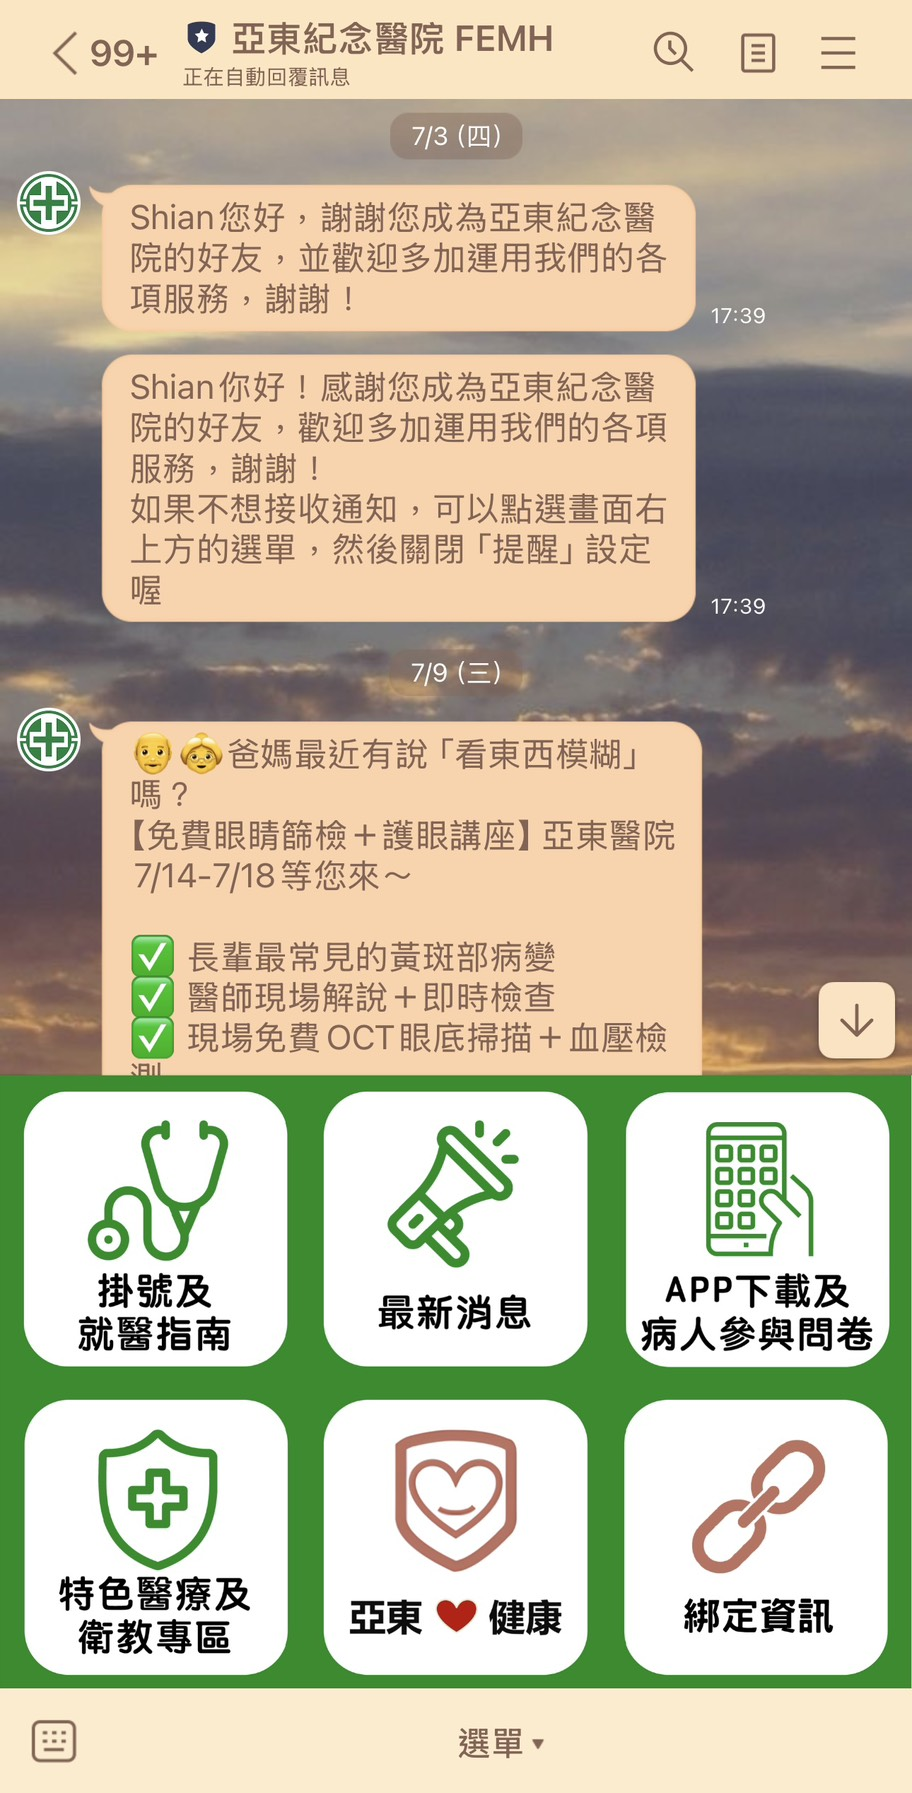
\includegraphics[width=0.2\textwidth]{../../images/line.jpg}
    \caption{Screenshot of the LINE system of Far Eastern Memorial Hospital, captured from the hospital’s official LINE account. The menu offers basic features such as booking appointments, viewing announcements, and linking personal information for customized services~\cite{femhline}.}
    \label{fig:line-service}
\end{figure}

These features are quite easy to use. However, each hospital has its own design and menu. Some functions even open in separate websites. There is no unified system, so it can be confusing for some patients, especially older people or those not familiar with technology.


\subsection{Other Existing Solutions}
% 內容...

\clearpage  % ← 這裡強制換頁


\clearpage
\section{Requirements}
\label{sec:requirements}
% requirements here

The system is primarily designed as a web-based platform for general hospital staff, specifically doctors and nurses, to facilitate interaction with patients. The core aim is to enable healthcare professionals to manage patient information, conduct remote consultations, and reduce the need for patients to visit the hospital in person.
While patients are also considered stakeholders of the system, the focus of the design and development process was placed on the needs of doctors and nurses. The decision was driven by the goal of reducing the administrative and operational workload for hospital staff, thereby improving efficiency within clinical workflows.

To ensure a functional and effective experience for hospital staff and patients, the system was designed to support a core set of features. These include secure user login and authentication for doctors and nurses, the ability to record patient vitals and view historical data trends, and an interface for remote consultation to minimise unnecessary hospital visits.
As the project was developed from scratch and targeted doctors, nurses, and patients, it required the collection of foundational requirements to support the intended clinical workflow. Based on input from our original client, Virtual Hospital Africa, we analysed their existing system and designed a new solution aligned with the vision of building a smart hospital.

Non-functional requirements were also considered throughout the development process. These included ensuring a responsive and mobile-friendly user interface, main-
taining data privacy through secure authentication and role-based access control, and optimising
performance for minimal load times to support real-time clinical usage. These system capabilities are closely aligned with the user stories
presented blew.

\vspace{1em}
% Adds vertical space before the table
\begin{table}[H]
% [H] makes the table stay exactly where it's written in the document
\centering
% Centers the table on the page
\renewcommand{\arraystretch}{1.4}
% Increases row height for better readability
\begin{tabular}{|p{2cm}|p{5.2cm}|p{5.2cm}|p{2cm}|}
% Defines a table with 4 columns of fixed widths
\hline
\textbf{As a...} & \textbf{I want...} & \textbf{So that...} & \textbf{Technical ability} \\
\hline
Doctor & To record and view patient vitals history & I can make more accurate clinical decisions based on patient trends & 3--5 \\
\hline
Doctor & To view patient contact information & I can conduct online or follow-up appointments to discuss test results or treatments & 3--5 \\
\hline
Nurse & To input vitals data easily through a form interface & I can reduce manual paperwork and save time during rounds & 2--4 \\
\hline
Patient & To view my previous visits and vitals data online & I can better understand my health condition over time & 2--3 \\
\hline
\end{tabular}
\caption{Smart Hospital User Stories Table} % Adds a caption under the table
\label{tab:user-stories}% Allows referencing the table elsewhere in the document
\end{table}

\vspace{1em}
% Adds space after the table

